\chapter{Code Architecture and Parallelism} \label{chapter:architecture-parallelism}

\section{Introduction}
\label{sect:introduction}
Accurate prediction of volcano plume development in a given time window requires resolution (very high particle counts) that can not be accomplished without parallel computing. Imposing  some types of boundary conditions (such as wind field, eruption boundary condition at the vent) requires dynamically adding and removing particles during simulation. This requires an efficient and flexible data management scheme. This chapter will present the architecture that enables efficient and flexible data managemnt and algorithms for solver parallelization.

Most implementations of the parallel SPH method presented to date are limited to standard SPH and benchmark problems like dam breaks, or relatively simple scenarios like breaking-waves, flooding, etc. Work on more complicated implementations is relatively rare. The demands of flexible data access are scarely addressed. Among existing CPU parallel SPH schemes, most of them focus on neighbor searching algorithms and dynamic load balancing. (eg. \citep{ferrari2009new, crespo2015dualsphysics}). Less attention has been paid to developing more flexible data management schemes. 
Fortunately, efficient and flexible data management strategies for parallel computing have been successfully implemented in mesh based methods (eg. \citep{laszloffy2000simple} for adaptive hp finite element method (FEM), and \citep{patra2005parallel} for finite volume method (FVM)). Motivated by these techniques developed for mesh based methods, we present a complete framework for parallelizing SPH program with the MPI standard allowing flexible and efficient data access.\\
Any implementation of SPH requires efficient searching and updating of neighbors during the simulation. Of the many possible choices we adopt the popular background grid method \citep{monaghan1985refined}, which is also used for domain decomposition. We refer to the elements of the background grid as buckets. 
As for the actual storage of data representing the physical quantities associated to each particle, different strategies have been adopted in existing implementations of SPH. 
In DualSPHysics \citep{crespo2015dualsphysics}, the physical quantities of each particle (position, velocity, density...) are stored in arrays, and the particles (and the arrays with particle data) are reordered following the order of the cells. It is not flexible enough to add, delete and especially access particles for such fixed-size arrays. \citet{ferrari2009new} adopted linked lists using pointers so that particles can be deleted or added during the simulation. Storage problems caused by fixed-size arrays are thereby also eliminated. We adopt hash tables to store pointers to objects of particles and buckets, which give us not only flexibility of deleting and adding of elements, but also quicker access compared with linked lists. A SFC-based index is adopted to give each particle and background bucket an unique identifier -- a strategy known to preserve some locality at minimal cost. The SFC based numbering strategy is further extended to include time step information so that particles added at the same position but different time will have different identifiers. 
We adopt an easy-programming scheme based on SFC \citep{patra1999efficient} to decompose the domain.

To the best of the author's knowledge, no current implementation of SPH has the feature of adjusting the computational domain based on simulation needs. For volcano plume simulation, this feature will greatly reduce computational cost by avoiding computing of uninfluenced fluids. This feature is accomplished by adding a scan function to monitor the outermost layer of the domain and turn ghost particles to real particles at the proper time thus effectively defining a halo domain with an almost optimally defined size.

\section{Workflow}
\begin{figure*}[!t]
\centering
\includegraphics[scale=0.43]{Chapter-5/Figures/Work_flow}
\hfil
\includegraphics[scale=0.43]{Chapter-5/Figures/Work_flow_adjust}
\caption{Workflow for SPH code. Figure to the left is the basic workflow. The right figure is the workflow that enables dynamic halo domain. These steps in organge box are newly added steps. Extra computational costs associated with these extra steps are discussed in section \ref{sec:effect-of-halo-domain}}
\label{fig:Work_flow}
\end{figure*}

In SPH, the domain is discretized by particles and the position of each particle is updated at every time step. The governing equations are estimated as sums over particles in a compact subdomain defined by the support of the kernel function. Only particles located within the support of the kernel function will interact. Thus, physical properties associated with the particle are updated based on its neighbors. A neighbor search therefore needs to be carried out before updating physical properties. Figure \ref{fig:Work_flow} shows the basic workflow of our SPH code, which includes three sections in the major updating loop: pre-updating section (neighbour searching and updating wall boundary conditions), physical quantities updating section and domain repartition section. Adding of new eruption ghost particles is carried out right after particle position updating in the updating section. Pressure outlet boundary condition is setup at initial condition setup step and dose need to update during simulation.
We use buckets, which contain all particles associated with a sub-domain (see Fig. \ref{fig:SFC_domain_decomposition}) 
and keep them stationary during the entire simulation, to reduce neighbour searching cost (since the search can now be restricted to only neighboring domains). No physical quantities are associated with bucket.

Domian is also partitioned based on the background mesh, whose elements are buckets containing the discretization points. Domain is decomposed by cutting SFC going through centroids of all buckets, as shown in Fig. \ref{fig:SFC_domain_decomposition}.
Data synchronization is carried out after every updating. Computational load of each subdomain is evaluated by summing up calibrated particle weights. Computational domain is redecomposed to restore load balance when necessary.
In current implementation, domain repartition is not carried after every time, instead, at an optimized interval.

The basic elements, particles and buckets, are identified by unique ID that generated based on SFC. All data are managed by hash tables, with external linked list to handle hash conflict. SFC is also used to decompose the computational domain.


\section{Data management and parallelization}
\subsection{SFC based indexing}
Our data structure starts from assigning each particle and bucket an identifier, we refer to it as a key, which should be unique throughout the simulation. The key for a bucket is determined by the centroid coordinate of the bucket while the key for a particle is determined by adding coordinates and time step of the particle. The map from coordinates to key is based on SFC \citep{sagan2012space} which maps a n-dimensional domain to a one dimensional sequence. The standard procedure for obtaining the SFC is: 
\begin{itemize}
\item Scale all coordinates in computational domain ($\textbf{X}^\prime$) into an $n$ dimensional unit hypercube $[0,1]^n $: $\textbf{X}^\prime \rightarrow \textbf{X}$, where $\textbf{X}$ represents coordinates in the hypercube.
\item Compute $k_r = h_n(\textbf{X})$. Where $h_n$ is the map $h_n: [0,1]^n \rightarrow [0,1]$. 
\item Convert $k_r$ to integer $k$ by multiplying $k_r$ with a large integer and removing decimal part.
\item Sort all keys to form a SFC sequence. The SFC represents a curve passing through all particles (or centroids of buckets).
\end{itemize}
%
\begin{figure*}[!t]
\centering
\includegraphics[scale=0.26]{Chapter-5/Figures/SFC_particles_buckets}
\hfil
\includegraphics[scale = 0.275]{Chapter-5/Figures/SFC_particles_buckets_partition}
\caption{The left figure shows SFCs passing all particles and buckets. The right figure shows an example of a domain decomposition based on the SFC of buckets.}
\label{fig:SFC_domain_decomposition}
\end{figure*}

Details for constructing the map $h_n$ can be found in \citep{patra1995problem}. These keys denote a simple addressing and ordering scheme for the data, i.e., a global index space for all the objects.

In some situations, new particles need to be added during the simulation. For example, new particles need to be added at the bottom of the eject vent (see Fig. \ref{fig:Particle_adding_with_link}). To assign distinct identifiers for particles added at the "same position" but at different time steps, we extend the SFC-based key to a time-dependent SFC based key by including date of birth of particles into their keys. The time-dependent SFC based key can be denoted as: $[k,t]$, where $t$ is the time step. The map $h_n$ will become:
\begin{equation}
h_n: [0,1]^n \times \textbf{T} \rightarrow [0,1] \times \textbf{N}
\end{equation}
Where $\textbf{T} \subset [0,\infty)$ is the time dimension, and $\textbf{N}=\lbrace 0, 1, 2, 3...\rbrace$.
To guarantee locality, sorting of particle keys is based on $k$, that is to say, particles with smaller $k$ always come before particles with larger $k$. For particles that have the same $k$, ordering will then depend on $t$. Figure \ref{fig:SFC_domain_decomposition} shows SFC ordering of buckets and particles in buckets. 
Several features of this indexing scheme are suitable for SPH:
\begin{itemize}
\item Guaranteed uniqueness of keys.
\item The key of each object is generated purely based on its own coordinates. When we add new objects on different processes, the key of each object can be generated fast and independently.
\item Objects that are located closely in the Euclidian space will also be close to each other in the one dimensional SFC key space in a mean sense. Since SPH particles only interact with their neighbors, geometric locality can be exploited for efficient access of data.
\item This type of key effectively generates a global address space. Globalism of key and conservation of spatial locality make it easy to partition the sorted key sequence and obtain a decomposition of the problem.
\end{itemize}

The (time-dependent) SFC based indexing plays central pivot role in the architecture. Besides creating unique ID efficiently and independently, SFC based domain decomposition helps preserve spatial locality making it very easy to design a hash function that preserve such locality in memory. The globalism of such indexing, which is also inherited in hash table, greatly simplifies complexity when moving elements around. As index generating (hence hashing) is independent and fast, creating/deleting of element are efficient and flexible.
All these features help keep the overall architecture breif, robust and sustainable.

\subsection{Data management strategies}
\subsubsection{Particle and bucket}
The most basic data structure of SPH are particles and buckets. Both are defined as C++ classes. Information that is contained in particle objects can be categorized into six categories: identifier (the key), affiliate(rank of the process that the particle belongs to), primitive variables (variables in governing equations, e.g. density, velocity), secondary variables (physical properties that can be computed from primitive variables, they are stored to avoid repeated computations, e.g., pressure and temperature), flags (indicators, such as indicator for ghost particle or real particle) and neighbor information (it is a vector of particle keys in our application). Similarly, information that is contained in a bucket object can also be categorized into different categories: identifier, affiliate, dimension information (maximum and minimum coordinates, boundary information), flags (indicators, such as guest indicator, which is used  to indicate whether the bucket belongs to another adjacent subdomain or not), neighbor information (keys of 27 neighbor buckets including its own key) and owned particles (it is a vector of particle keys in our application).
Using of several independent flags creates a multiple-dimensional categorization space which enables flexible elements categorization simplifing algorithms.
Objects of particles and buckets are then accessed through hash tables.

\subsubsection{Hash table and hash collision}
Several data structures have been considered for actual data storage. Vector and array can guarantee efficicent and flexible element access while inserting of new elements is either expensive or not allowed. List type of data structure allows flexible and efficient new element insert but element access is expensive ($(O(n)$).
Hash table guarantees fast element access ($(O(1)$) while allows flexible and efficient new element insert. Hashmap also also allows allows flexible and efficient new element insert, but its element access is a little more expensive($(O(logn)$). We finally choose to use hash table, which is essentially a chunck of memory with many slots. The pointer to certain element object is stored in one slot. Based on the keys of data, the address-calculator(hashing) function determines in which slot the data should be stored:
\begin{equation}
Index = hash(key)
\end{equation}

Data in a hash table can be accessed with time complexity of $O(1)$ when there is no hash collision. One way to handle hash collisions is to use an additional sorted vector attached to the hash table. When several keys hash to the same index, a vector will be created. The vector is sorted based on keys so that a binary search (with an average time complexity of $O(log n)$) can be used to find the correct position for adding, deleting or retrieving of data. Another option is using an additional linked list which is more flexible in memory allocation but slower in searching $(O(n)$). In addition, pointer based memory accessing of linked lists will greatly slow down the efficiency of data access for long linked lists. Choosing the proper way to handle hash conflicts greatly depends on the problem itself. For volcano plume simulation, new particles are added at the bottom of the eruption vent (see Fig. \ref{fig:Particle_adding_with_link}), making the linked list a better choice. Pointers to these new particles will be stored in external linked lists as shown in Fig. \ref{fig:Particle_adding_with_link}.
\begin{figure}
\centering
{\includegraphics[scale=0.42]{Chapter-5/Figures/Particle_adding_with_link}}
{\caption{Non-uniform distribution of particles in the $[0,1]^n \times \textbf{T}$ space due to adding of new particles at a small area of the whole domain.}
\label{fig:Particle_adding_with_link}}
\end{figure}

\begin{figure}
\centering
{\includegraphics[scale=0.45]{Chapter-5/Figures/int_bar}}
{\caption{The influence of different load balance check intervals on simulation time. The bar values are the extra simulation time in log scale. The optimized interval is 3s.}
\label{fig:check_int}}
\end{figure}

For time-independent keys, the hash function can be a simple function like:
\begin{equation}
Index= \frac{Key - Min\,Key}{Max\,Key - Min\,Key} 
\times Hash\,Table\,Size 
\label{eq:hash_function}
\end{equation}

One natural way to hash time-dependent keys $[k,t]$ is to convert the two elements in the key into one number taking $k$ as the higher digit and $t$ as the lower digit of the large number. However, for volcano plume simulation, only ghost particles for eruption boundary condition will be successively added at the same place: the bottom of the vent. That is to say, particles are distributed non-uniformly in the $[0,1]^n \times \textbf{T}$ space as shown in Fig. \ref{fig:Particle_adding_with_link}. To avoid a non-uniform sparse hash table and conserve spatial locality, we only plug the first number, $k$, of the key, $[k,t]$, into the hashing function, Eq. (\ref{eq:hash_function}). All particles with the same birth location will hash to the same slot and be handled by external linked lists.

\subsection{Domain decomposition and load balancing strategy}
\label{sect:load_balance}
\subsubsection{Weighted work load} \label{sec:Weighted_work_load}
Particles in our problem can be categorized into four types: real particles, wall ghost particles, pressure ghost particles and eruption ghost particles. Ghost particles are for imposition of corresponding boundary conditions (See Fig. \ref{fig:Plume}). As different types of particles involve different amount of computational work, shown by table \ref{tab:Computational_cost_steps}, we assign different work load weights for different types of particles based on profiling data. Instead of simply using number of contained particles as work load for buckets, work load of each bucket is determined by summing up work load weights of all particles within the bucket.
\begin{equation}
W^{bucket} = \sum_i^{N^{particle}} W_i^{particle}
\label{eq:work-load-bucket}
\end{equation}
where $N^{particle}$ is total number of particles contained by the bucket. $W_i^{particle}$ is weight of particle, depending on particle type (see Table \ref{tab:Computational_cost_steps}).
The SFC of buckets now becomes a weighted sequence. Domain decomposition is conducted by cutting the weighted SFC of buckets into pieces.

\begin{figure}
\centering
%\CenterFloatBoxes
%\ttabbox
%{	  
	  \begin{tabular}{lrrrrrr}
	    \hline
	    Step & Cost ($ms$) & Real & wall & eruption & pressure\\
	    \hline
	    neighbor search & 0.41 & Yes & No & No & No \\
	    update momentum and energy & 0.70 & Yes & No & No & No\\
	    update density & 0.42 & Yes & No & No & No \\
	    update position & 0.01 & Yes & No & Yes &  No\\
	    velocity filtering& 0.43 & Yes & No & No & No\\
	    apply wall boundary condition     & 0.75 & No & Yes & No & No\\
	    summation ($ms$) & - & 1.97 & 0.75 & 0.01 & 0.00\\
	    \hline
	  \end{tabular}
%}
{\caption{Computational cost per particle for different steps}	}
\label{tab:Computational_cost_steps}
\end{figure}

\subsubsection{Domain decomposition and dynamic load balancing}
Figure \ref{fig:SFC_domain_decomposition} shows how the domain is decomposed based on partition of the SFC of buckets. The particles are automatically split into several groups along with buckets that contain them. As the SFC of buckets is a curve in 3D space, partition of this curve will automatically lead to 3D domain decomposition. Each piece of the SFC after partitioning, which will be calculated by each processor, should then have a balanced total work load. That is to say:
\begin{equation}
W^{process}_1 \approx W^{process}_2 ... \approx W^{process}_i ...\approx W^{process}_{N^{process}}
\label{eq:work-load-balance}
\end{equation}
where $N^{process}$ is total number of processors, work load of each processor is calculated according to Eq. (\ref{eq:work-load-process}).
\begin{equation}
W^{process} = \sum_i^{N^{bucket}} W_i^{bucket}
\label{eq:work-load-process}
\end{equation}
where the work load of each bucket is evaluated based on Eq.(\ref{eq:work-load-bucket}).

As some of the neighbor particles reside in other partitions, a set of ``guest'' particles and buckets are used to synchronize data across partitions. To minimize communications, data is synchronized only after updating of physical quantities and positions or after repartition. Data associated with a single particle (or bucket) are first packed up before send out and then unpacked after receiving. In addition, not all information contained by element (bucket or particles) is packed. For example, secondary variables and neighbour information of particles are not send out. In this way, the amount of data that need communicate is reduced. Packed data will be loaded onto a bus (an array whose elements are packed buckets or particles) and send out once. Non-blocking MPI communications is adopted to reduce communication overhead.

Movement of particles, adding of new particles, and adjustments of domain will lead to significant load imbalance between processes. To restore load balance, computational load is monitored at a given interval which is optimized based on numerical experiments (see details in section \ref{sec:numerical-tests-computation}). Repartitioning is carried out when load imbalance is larger than a given tolerance.

\section{Dynamic halo domain} 
For plume simulation and similar phenomena, where some fluid ejects into a stationary fluid and gets mixed, the stationary fluid must be represented.
A lot of CPU time will be spent on computing associated with these stationary particles. If simulation of stationary particles can be avoided, the computational cost will be greatly reduced.
We propose a simple strategy to add such a feature to our code with low computational cost. We add a scan function to monitor the outermost layer of the domain. When the ejected fluid reaches the boundary of the current domain, pressure ghost particles (light blue particles in the right figure of Fig. \ref{fig:Plume}) will be turned to real particles (red particles in the right figure of Fig. \ref{fig:Plume}) and then add a new layer of pressure ghost particles for pressure boundary conditions. Wall ghost particles (grey particles in the right figure of Fig. \ref{fig:Plume}) will also be added when necessary. The original workflow is modified to enable such a feature. The modified workflow is shown on the right in Fig. \ref{fig:Work_flow}).

An involvement flag is added to particle class to distinguish different states of involvement. Particles are categorized into three groups based on the value of the involvement flag: involved, potentially involved, and not involved. The involved particles are particles that have already been affected by the mixing. The potentially involved particles are particles that have not been involved in mixing but are adjacent to involved particles and will thus be involved in the near future. 
All communication and computation associated with uninvolved particles can be ignored. That is to say, only potential involved and involved particles need to be simulated.
As simulation progresses, the ejected fluid will reach a larger area and more and more particles will be influenced. When originally stationary air is influenced by erupted material, the mass fraction of the erupted material will increase from zero to a positive value. So we can determine whether a particle should turn to involved status based on whether the mass fraction of that particle is larger than a given threshold ($10^{-5} $ in our simulation) or not. Based on such criteria, any real particles of phase 2 (erupted material) are qualified to be involved particles.  Particles of phase 1 (air) are also qualified to be involved particles if they are inside of the plume or close to the margin of plume. Other physical properties, like velocity, might also serve as alternative ``switch criteria''. Switching of particles from potentially involved to involed status is carried out right after mass fraction updating (the ``density update" step in left figure of Fig. \ref{fig:Work_flow}).

A similar scheme is also deployed for buckets resulting in a categorization of buckets. The additional complexity is that potentially involved ghost particles must also be taken into accounted. The switch criteria for bucket from potentially involved to involved is based on the fact whether the bucket contains any involved particles. Switching of bucket from potentially involved to involved is carried out in the a newly added step in the workflow, the ``Scan the Most Outside Layer
Buckets \& Return Adapt Indicator" step.

By implementing the algorithm of dynamics halo domain presented above, the computational domain grows dynamically during simulation. Figure \ref{fig:Plume} shows a cross-sectional view of a typical computational domain during simulation. As can be seen, the plume just fit into the computational domain, which has irregular geometry.

\begin{figure*}[!t]
\centering
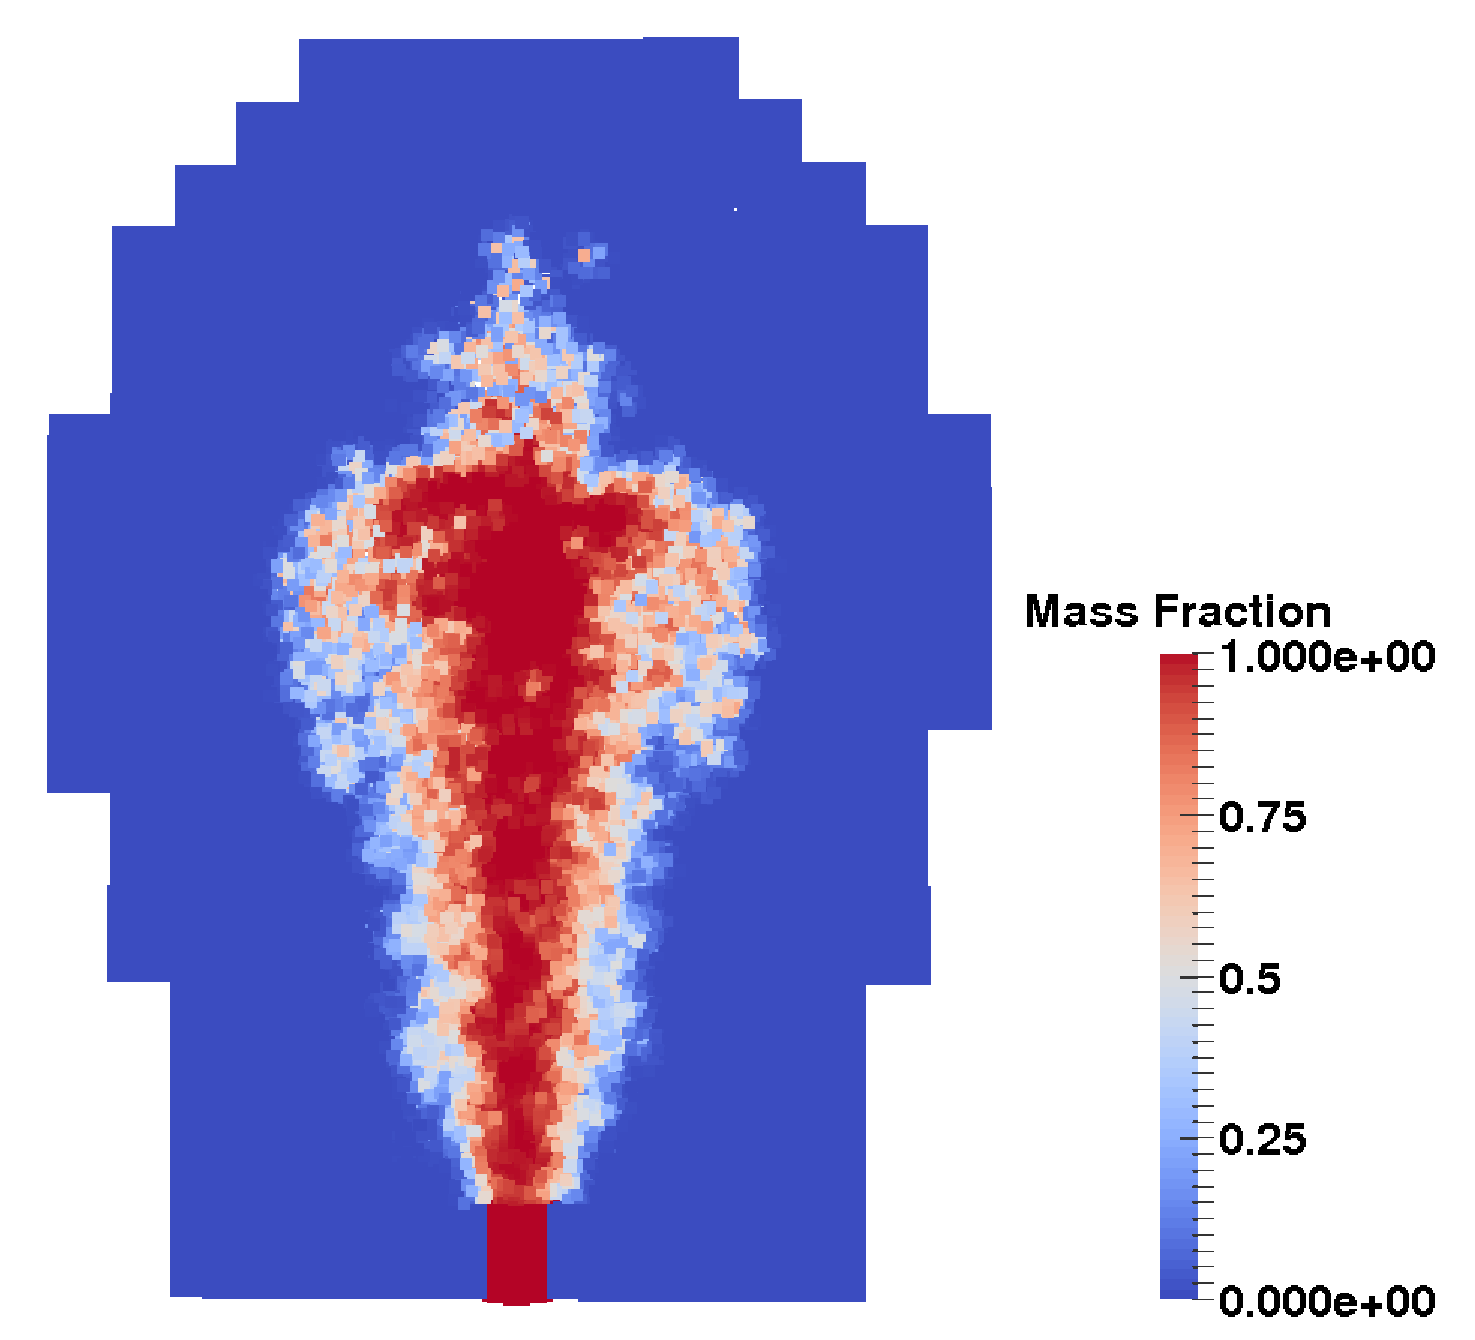
\includegraphics[scale=0.28]{Chapter-5/Figures/Plume_simulation}
\hfil
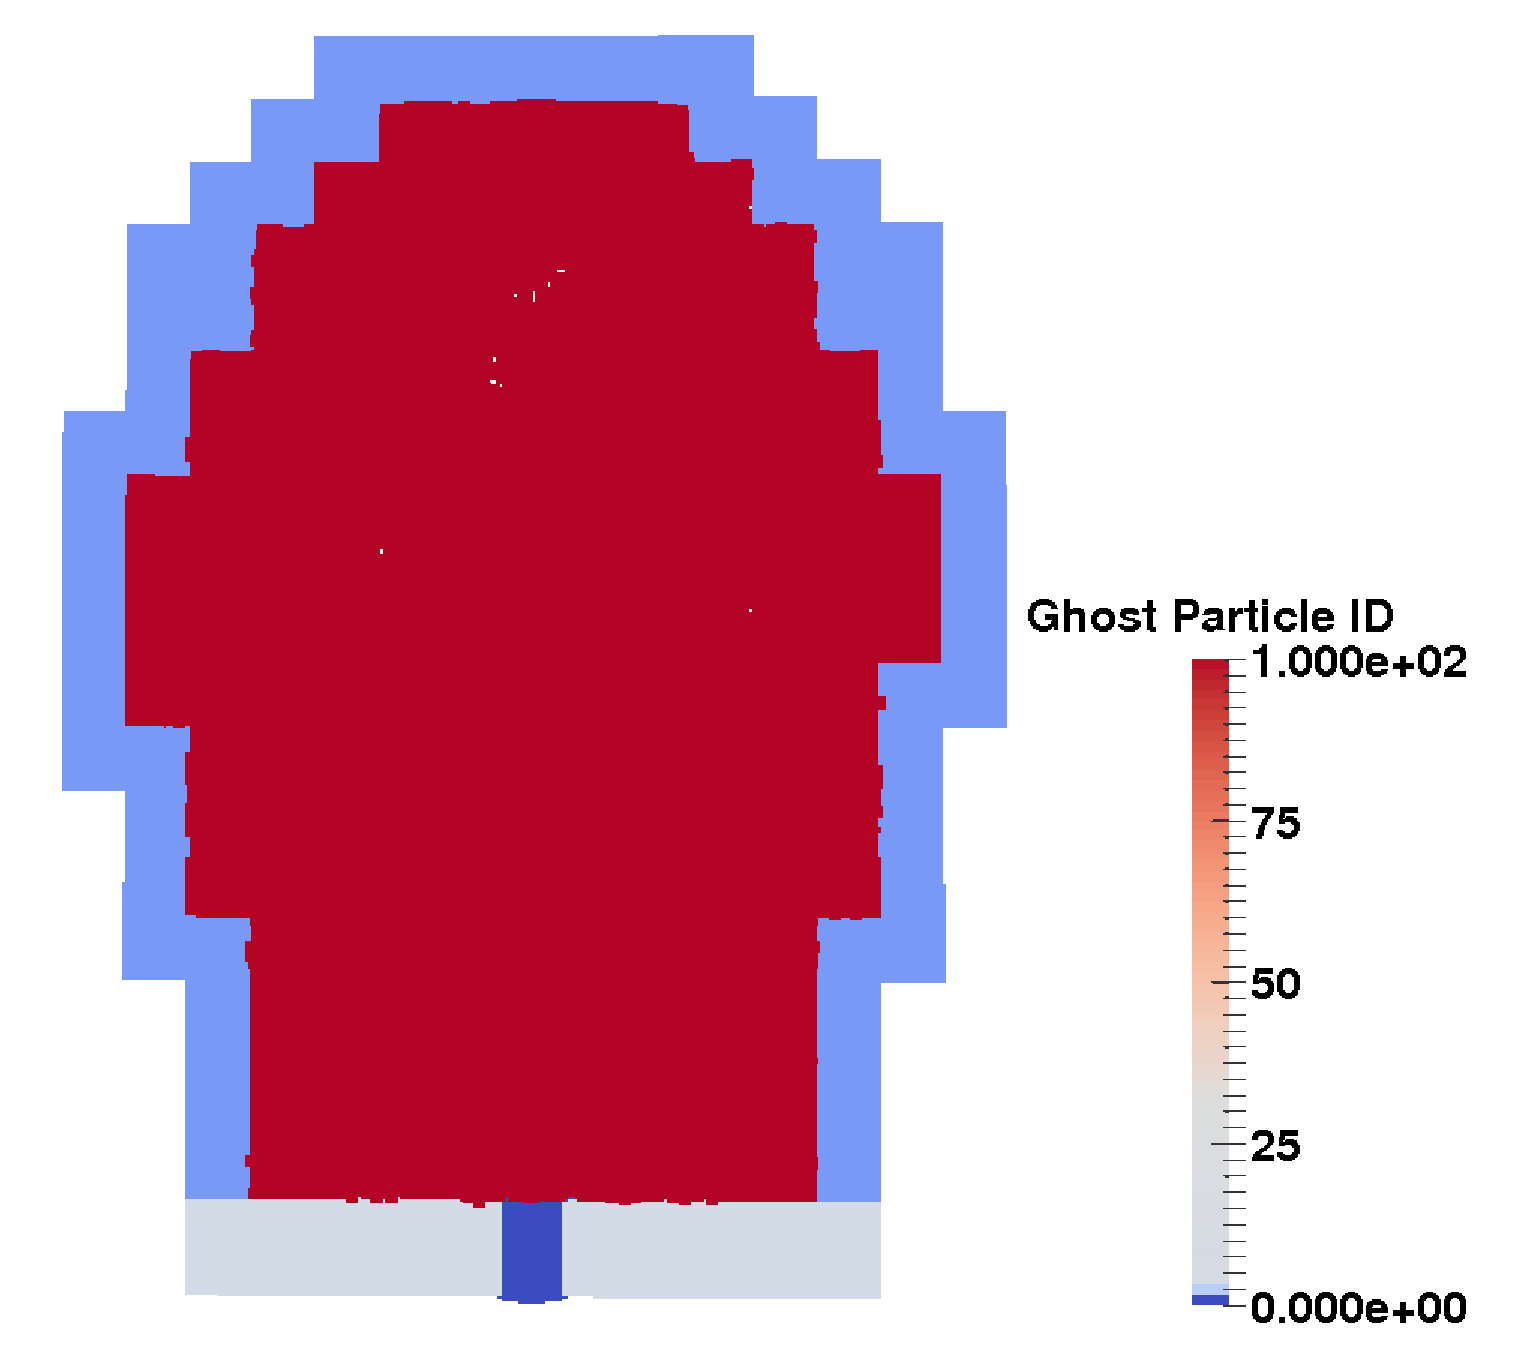
\includegraphics[scale=0.28]{Chapter-5/Figures/Boundary-condition}
\caption{The left figure shows contour of mass fraction at specific time during simulation. The volcano plume is represented by high mass fraction region. The right figure is a cross-section view of the computational domain at corresponding time.}
\label{fig:Plume}
\end{figure*}

\section{Numerical test} \label{sec:numerical-tests-computation}
Numerical tests are carried out in this section. Tests on overall parallel performance, including the weak scalability and strong scalability, are presented first. The effect, in terms of computational effiency, of several special algorithms are demonstrated, including the optimized load balance check interval, calibrated particle weights and the dynamic halo domain.

\subsection{Scalability test}
\begin{figure*}[!t]
\centering
\includegraphics[scale=0.31]{Chapter-5/Figures/strong_scale}
\hfil
\includegraphics[scale=0.31]{Chapter-5/Figures/strong_scale_zoom}
\hfil
\includegraphics[scale=0.31]{Chapter-5/Figures/weak_scale}
\caption{The left figure shows strong scalability tests result. middle figure is the zoomed view of first one. It is obviously shown that strong scalability is better when the problem size is larger. The right figure is weak scalability test results}
\label{fig:2cases_efficiency}
\end{figure*}

Experiments have been carried out on the computational cluster of Center for Computational Research (CCR) at Buffalo. 
The compute servers have 12 cores (two Xeon E5645 processors per server) running at 2.40GHz clock rate with 4GB memory per core on a Q-Logic Infiniband network. Main memory and level 3 cache are shared on each node. The simulation domain is a box with initial dimension $[-4.8km, 4.8km]\times [-4.8km, 4.8km] \times [0km, 6km]$ for case 1 and $[-10km, 10km]\times [-10km, 10km] \times [0km, 5km]$ for case 2. The smoothing length (we set initial intervals between particles equal to smoothing length) equals to 200m and 100m respectively for test case 1 and test case 2. So the computational work load of test case 2 is larger than that of the test case 1. The simulations run for 20s physical time.  Parallel speed up is shown in Fig. \ref{fig:2cases_efficiency}. Test case 2 shows better speed up than test case 1 which implies that strong scalability can be improved by increasing total amount of work load.
The weak scalability test is conducted with the same initial domain as test case 1 and various smoothing length. Each simulation runs for 400 time steps. The average number of real particles for each process keeps constant at $25900$, so the average work load for each processor is approximately constant. 
Right side figure in Fig \ref{fig:2cases_efficiency} shows the timing of a weak scalability test.

\subsection{Effect of workload check interval and calibrated particle weight} \label{sec:effect-of-workload-check-interval}
\begin{figure}
\centering
%\CenterFloatBoxes
%\ttabbox
{	  
	  \begin{tabular}{lrrrr}
	    \hline
	    Physical time & 10 s & 20s & 30 s & 40 s \\
	    \hline
	    Same weight & 1141.7 & 4119.4 & 10371.0 & 12453.7\\
	    Different weights & 1108.2 & 4057.0 & 10281.5 & 12166.3\\
	    \hline
	  \end{tabular}
}
{\caption{Simulation time for the same particle weight and different particle weights at different physical times.}}
\label{tab:same_diff_particle_weight}
\end{figure}
In section \ref{sect:load_balance}, we proposed to use different particle weights for different types of particles when estimate the workload of buckets. The effect of using different particle weight is demonstrated in table \ref{tab:same_diff_particle_weight}. The simulation time is reduced by using different particle weights. However, the amount of time that is reduced is not as significant as we expected. One possible explanation is that real particles are the major population, so the load imbalance caused by assigning improper weight values to ghost particles is small.

The best load balance check interval is calibrated based on a series of simulations with different load balance scan intervals. From 0 - 50 seconds physical time, the interval of 1 second shows a better load balance than interval of 2 seconds. However, for the simulation of 50 - 100 seconds, interval of 2 seconds is better. This implies that loss of load balance accumulates faster and requires a more frequent re-decomposition of domain at the early stages of simulation. This is consistent with the plume development process: the domain grows quickly at the beginning as erupted material ejects into the environment and spreads. Afterwards, the spreading speed of the front edge slows down due to viscosity and momentum exchange leading to slowing down of domain growth. We need to emphasize that, these optimized parameters, including weights of particles and load balance checking interval, are case sensitive and need to be re-calibrated for different applications and hardware architecture.

\subsection{Effect of dynamic halo domains} \label{sec:effect-of-halo-domain}
\begin{figure}
\centering
%\CenterFloatBoxes
%\begin{floatrow}
%\ttabbox
{	  
    \begin{tabular}{lrr}
    \hline
    Functions & Total time (s) & Called times\\
    	\hline
    UPME & 2954.8 & 201 \\
    UPP & 38.55 &  201 \\
    ADPP & 21.51 & 3 \\
    ADWP  & 8.88 & 3 \\
    SWCH & 0.08 &  2 \\
    SCN  & 7.72 & 201 \\
    \hline
  \end{tabular}
}
{\caption{Computational work load of extra steps for domain adjusting. SWCH represents step that switch pressure ghost particle to real particle, ADPP is short for adding new pressure ghost particles, ADWP represents adding wall ghost particles, SCN is short for scanning the outmost layer of the domain.  Momentum and energy update (UPME) and position update (UPP) also included for comparison.}
\label{tab:Computational_cost_doamin_adj}}
\centering
{\includegraphics[scale=0.5]{Chapter-5/Figures/adj_vs_no}}
{\caption{The figure on the top shows execution time without domain adjusting, the figure on the bottom shows execution time with domain adjusting. Different bins represent execution time up to specific physical time indicated by horizontal axis.}
\label{fig:adj_vs_no}}
%\end{floatrow}
\end{figure}
For the test problem, the volcano plume finally reaches to a region of $[-10km \,\,\, 10km] \times [-10km\,\,\,10km] \times [0km\,\,\,20km]$ after around 300 seconds of eruption. When numerical simulation goes up to 90 seconds, the plume is still within a region of $[-3km\,\,\,3km] \times [-3km\,\,\,3km] \times [0km\,\,\,6km]$. This implies that adjusting of domain can avoid computing large number of uninfluenced particles, especially for the early stages of simulation. On the other hand, additional functions (see Fig. \ref{fig:Work_flow}) for domain adjusting will add extra computational cost. Table \ref{tab:Computational_cost_doamin_adj} shows the extra computational cost corresponding to these functions. Profiling data for momentum and energy update (UPME) and position update (UPP) is also included in the table for the purpose of comparison. As we can see from the table, the cost of SCN is even smaller than UPP function, which is the cheapest function (as shown in table \ref{tab:Computational_cost_steps}) in the regular workflow (see Fig. \ref{fig:Work_flow}). The other three functions, ADPP, ADWP and SWCH, are only called a few times during the simulation, and as a consequence, the extra computational cost due to them are negligible. To summarize, the additional cost caused by the domain adjusting functions is ignorable.
Figure \ref{fig:adj_vs_no} shows that simulation time of the test problem is greatly reduced when we adopt the domain adjusting strategy in our code.

\section{Conclusion}
We developed data management strategies for a MPI-parallel implementation of the SPH method to simulate volcano plumes. Neighbor searching and domain decomposition is based on the background grid. A SFC based index scheme is adopted to identify buckets and time-dependent SFC keys are used as identifiers for particles. 
Hash tables with external linked lists are adopted for accessing particles and buckets data. Based on calibrated particle weights, a dynamic load balance strategy is developed by checking load balance and re-decomposing the domain at an optimized interval. The performance of the code was further improved by several factors by adjusting the computational domain during simulation.
Overall we obtain good scalability and performance.

The flexibility of our data access methodology enables implementing mesh-free methods for solving more complicated problems and using more advanced techniques, such as dynamic particle splitting techniques \citep{vacondio2012accurate, feldman2007dynamic}, which will give higher resolution at the area of interest by splitting one large particle to several smaller ones. The data structure, particle and bucket indexing strategies, domain decomposition, dynamic load balancing method and domain adjusting strategies in present work can be adopted to other mesh-free methods (not just SPH).
